% !Mode:: "TeX:UTF-8"
% !TEX program = xelatex

%%%%%%%%%% Port for macOS %%%%%%%%%%%
% Modified: Qin Yubo

\def\usewhat{xelatex}
\documentclass[10pt,openany,oneside]{ctexbook}
                                                     % 本科生毕业论文通常采用单页排版
% !Mode:: "TeX:UTF-8"
%  Authors: 张井   Jing Zhang: prayever@gmail.com     天津大学2010级管理与经济学部信息管理与信息系统专业硕士生
%           余蓝涛 Lantao Yu: lantaoyu1991@gmail.com  天津大学2008级精密仪器与光电子工程学院测控技术与仪器专业本科生

%%%%%%%%%% Package %%%%%%%%%%%%
\usepackage{CJK}
\usepackage{lmodern}
\usepackage[T1]{fontenc}
\usepackage{graphicx}                       % 支持插图处理
\usepackage[a4paper,text={146.4true mm,239.2 true mm},top= 26.2true mm,left=31.8 true mm,head=6true mm,headsep=6.5true mm,foot=16.5true mm]{geometry}
                                            % 支持版面尺寸设置
\usepackage[squaren]{SIunits}               % 支持国际标准单位

\usepackage{titlesec}                       % 控制标题的宏包
\usepackage{titletoc}                       % 控制目录的宏包
\usepackage{fancyhdr}                       % fancyhdr宏包 支持页眉和页脚的相关定义
%\usepackage{ctex}                     % 支持中文显示
\usepackage{CJKpunct}                       % 精细调整中文的标点符号
\usepackage{color}                          % 支持彩色
\usepackage{amsmath}                        % AMSLaTeX宏包 用来排出更加漂亮的公式
\usepackage{amssymb}                        % 数学符号生成命令
\usepackage[below]{placeins}    %允许上一个section的浮动图形出现在下一个section的开始部分,还提供\FloatBarrier命令,使所有未处理的浮动图形立即被处理
\usepackage{multirow}                       % 使用Multirow宏包,使得表格可以合并多个row格
\usepackage{booktabs}                       % 表格,横的粗线;\specialrule{1pt}{0pt}{0pt}
\usepackage{longtable}                      % 支持跨页的表格。
\usepackage{tabularx}                       % 自动设置表格的列宽
\usepackage{subfigure}                      % 支持子图 %centerlast 设置最后一行是否居中
\usepackage[subfigure]{ccaption}            % 支持子图的中文标题
\usepackage[sort&compress,numbers]{natbib}  % 支持引用缩写的宏包
\usepackage{enumitem}                       % 使用enumitem宏包,改变列表项的格式
\usepackage{calc}                           % 长度可以用+ - * / 进行计算
\usepackage{txfonts}                        % 字体宏包
\usepackage{bm}                             % 处理数学公式中的黑斜体的宏包
\usepackage[amsmath,thmmarks,hyperref]{ntheorem}  % 定理类环境宏包,其中 amsmath 选项用来兼容 AMS LaTeX 的宏包
\usepackage{CJKnumb}                        % 提供将阿拉伯数字转换成中文数字的命令
\usepackage{indentfirst}                    % 首行缩进宏包
\usepackage{CJKutf8}                        % 用在UTF8编码环境下,它可以自动调用CJK,同时针对UTF8编码作了设置
%\usepackage{hypbmsec}                      % 用来控制书签中标题显示内容
\newcommand{\tabincell}[2]{\begin{tabular}{@{}#1@{}}#2\end{tabular}}
\usepackage{xcolor}
%支持代码环境
\usepackage{listings}
\lstset{numbers=left,
language=[ANSI]{C},
numberstyle=\tiny,
extendedchars=false,
showstringspaces=false,
breakatwhitespace=false,
breaklines=true,
captionpos=b,
keywordstyle=\color{blue!70},
commentstyle=\color{red!50!green!50!blue!50},
frame=shadowbox,
rulesepcolor=\color{red!20!green!20!blue!20}
}
%支持算法环境
\usepackage[boxed,ruled,lined]{algorithm2e}
\usepackage{algorithmic}

\usepackage{array}
\newcommand{\PreserveBackslash}[1]{\let\temp=\\#1\let\\=\temp}
\newcolumntype{C}[1]{>{\PreserveBackslash\centering}p{#1}}
\newcolumntype{R}[1]{>{\PreserveBackslash\raggedleft}p{#1}}
\newcolumntype{L}[1]{>{\PreserveBackslash\raggedright}p{#1}}

\def\atemp{xelatex}\ifx\atemp\usewhat
\usepackage[unicode,
            pdfstartview=FitH,
            bookmarksnumbered=true,
            bookmarksopen=true,
            colorlinks=false,
            pdfborder={0 0 1},
            citecolor=blue,
            linkcolor=red,
            anchorcolor=green,
            urlcolor=blue,
            breaklinks=true
            ]{hyperref}
\fi
                                % 定义本文所使用宏包
\graphicspath{{figures/}}                            % 定义所有的图像文件在 figures 子目录下
\begin{document}                                     % 开始全文
% !Mode:: "TeX:UTF-8"
%  Authors: 张井   Jing Zhang: prayever@gmail.com     天津大学2010级管理与经济学部信息管理与信息系统专业硕士生
%           余蓝涛 Lantao Yu: lantaoyu1991@gmail.com  天津大学2008级精密仪器与光电子工程学院测控技术与仪器专业本科生

%%%%%%%%%%%%%%%%% Fonts Definition and Basics %%%%%%%%%%%%%%%%%
%\newcommand{\song}{\CJKfamily{song}}    % 宋体
%\newcommand{\fs}{\CJKfamily{fs}}        % 仿宋体
%\newcommand{\kai}{\CJKfamily{kai}}      % 楷体
%\newcommand{\hei}{\CJKfamily{hei}}      % 黑体
%\newcommand{\li}{\CJKfamily{li}}        % 隶书
\newcommand{\song}{\songti}    % 宋体
\newcommand{\fs}{\fangsong}        % 仿宋体
\newcommand{\kai}{\kaishu}      % 楷体
\newcommand{\hei}{\heiti}      % 黑体
\newcommand{\li}{\lishu}        % 隶书
\newcommand{\biaotizihao}{\fontsize{32pt}{32pt}\selectfont}
\newcommand{\yihao}{\fontsize{26pt}{26pt}\selectfont}       % 一号, 单倍行距
\newcommand{\xiaoyi}{\fontsize{24pt}{24pt}\selectfont}      % 小一, 单倍行距
\newcommand{\erhao}{\fontsize{22pt}{1.25\baselineskip}\selectfont}       % 二号, 1.25倍行距
\newcommand{\xiaoer}{\fontsize{18pt}{18pt}\selectfont}      % 小二, 单倍行距
\newcommand{\sanhao}{\fontsize{16pt}{16pt}\selectfont}      % 三号, 单倍行距
\newcommand{\xiaosan}{\fontsize{15pt}{15pt}\selectfont}     % 小三, 单倍行距
\newcommand{\sihao}{\fontsize{14pt}{14pt}\selectfont}       % 四号, 单倍行距
\newcommand{\xiaosi}{\fontsize{12pt}{12pt}\selectfont}      % 小四, 单倍行距
\newcommand{\wuhao}{\fontsize{10.5pt}{10.5pt}\selectfont}   % 五号, 单倍行距
\newcommand{\xiaowu}{\fontsize{9pt}{9pt}\selectfont}        % 小五, 单倍行距

%\CJKtilde  % 重新定义了波浪符~的意义
% JUST DON'T USE CJK
% 使用 ctexbook 之后已无必要
\newcommand\prechaptername{第}
\newcommand\postchaptername{章}

\punctstyle{hangmobanjiao}             % 调整中文字符的表示,行内占一个字符宽度,行尾占半个字符宽度

% 调整罗列环境的布局
\setitemize{leftmargin=3em,itemsep=0em,partopsep=0em,parsep=0em,topsep=-0em}
\setenumerate{leftmargin=3em,itemsep=0em,partopsep=0em,parsep=0em,topsep=0em}

% 避免宏包 hyperref 和 arydshln 不兼容带来的目录链接失效的问题。
\def\temp{\relax}
\let\temp\addcontentsline
\gdef\addcontentsline{\phantomsection\temp}

% 自定义项目列表标签及格式 \begin{publist} 列表项 \end{publist}
\newcounter{pubctr} %自定义新计数器
\newenvironment{publist}{%%%%%定义新环境
\begin{list}{[\arabic{pubctr}]} %%标签格式
    {
     \usecounter{pubctr}
     \setlength{\leftmargin}{2.5em}   % 左边界 \leftmargin =\itemindent + \labelwidth + \labelsep
     \setlength{\itemindent}{0em}     % 标号缩进量
     \setlength{\labelsep}{1em}       % 标号和列表项之间的距离,默认0.5em
     \setlength{\rightmargin}{0em}    % 右边界
     \setlength{\topsep}{0ex}         % 列表到上下文的垂直距离
     \setlength{\parsep}{0ex}         % 段落间距
     \setlength{\itemsep}{0ex}        % 标签间距
     \setlength{\listparindent}{0pt}  % 段落缩进量
    }}
{\end{list}}

\makeatletter
\renewcommand\normalsize{
  \@setfontsize\normalsize{10.5pt}{10.5pt} % 小四对应 12 pt
  \setlength\abovedisplayskip{4pt}
  \setlength\abovedisplayshortskip{4pt}
  \setlength\belowdisplayskip{\abovedisplayskip}
  \setlength\belowdisplayshortskip{\abovedisplayshortskip}
  \let\@listi\@listI}
\def\defaultfont{\renewcommand{\baselinestretch}{1.63}\normalsize\selectfont} % 设置行距

\renewcommand{\CJKglue}{\hskip -0.1 pt plus 0.08\baselineskip} % 控制字间距,使每行 34 个汉字
\makeatother

%%%%%%%%%%%%% Contents %%%%%%%%%%%%%%%%%
\renewcommand{\contentsname}{目\qquad 录}
\setcounter{tocdepth}{2} % 控制目录深度
% 使用 ctexbook 之后已无必要
%\titlecontents{chapter}[2em]{\vspace{.5\baselineskip}\xiaosan\song}
             %{\prechaptername\CJKnumber{\thecontentslabel}\postchaptername\qquad}{}
             %{\hspace{.5em}\titlerule*[10pt]{$\cdot$}\sihao\contentspage}
\titlecontents{chapter}[2em]{\vspace{.5\baselineskip}\xiaosan\song}
             {\thecontentslabel\qquad}{}
             {\hspace{.5em}\titlerule*[10pt]{$\cdot$}\sihao\contentspage}
\titlecontents{section}[3em]{\vspace{.25\baselineskip}\sihao\song}
             {\thecontentslabel\quad}{}
             {\hspace{.5em}\titlerule*[10pt]{$\cdot$}\sihao\contentspage}
\titlecontents{subsection}[4em]{\vspace{.25\baselineskip}\sihao\song}
             {\thecontentslabel\quad}{}
             {\hspace{.5em}\titlerule*[10pt]{$\cdot$}\sihao\contentspage}

%%%%%%%%%% Chapter and Section %%%%%%%%%%%%%
\setcounter{secnumdepth}{4}
\setlength{\parindent}{2em}
\renewcommand{\chaptername}{\prechaptername\CJKnumber{\thechapter}\postchaptername}
\titleformat{\chapter}{\centering\xiaosan\song}{\hei\chaptername}{2em}{}
\titlespacing{\chapter}{0pt}{0.1\baselineskip}{0.8\baselineskip}
\titleformat{\section}{\sihao\hei}{\thesection}{1em}{}
\titlespacing{\section}{0pt}{0.15\baselineskip}{0.25\baselineskip}
\titleformat{\subsection}{\sihao\hei}{\thesubsection}{1em}{}
\titlespacing{\subsection}{0pt}{0.1\baselineskip}{0.3\baselineskip}
\titleformat{\subsubsection}{\sihao\hei}{\thesubsubsection}{1em}{}
\titlespacing{\subsubsection}{0pt}{0.05\baselineskip}{0.1\baselineskip}

%%%%%%%%%% Table, Figure and Equation %%%%%%%%%%%%%%%%%
\renewcommand{\tablename}{表}                                     % 插表题头
\renewcommand{\figurename}{图}                                    % 插图题头
\renewcommand{\thefigure}{\arabic{chapter}-\arabic{figure}}       % 使图编号为 7-1 的格式 %\protect{~}
\renewcommand{\thesubfigure}{\alph{subfigure})}                   % 使子图编号为 a) 的格式
\renewcommand{\thesubtable}{(\alph{subtable})}                    % 使子表编号为 (a) 的格式
\renewcommand{\thetable}{\arabic{chapter}-\arabic{table}}         % 使表编号为 7-1 的格式
\renewcommand{\theequation}{\arabic{chapter}-\arabic{equation}}   % 使公式编号为 7-1 的格式
\newcommand{\ud}{\mathrm{d}}

%%%%%% 定制浮动图形和表格标题样式 %%%%%%
\makeatletter
\long\def\@makecaption#1#2{
   \vskip\abovecaptionskip
   \sbox\@tempboxa{\centering\wuhao\song{#1\qquad #2} }
   \ifdim \wd\@tempboxa >\hsize
     \centering\wuhao\song{#1\qquad #2} \par
   \else
     \global \@minipagefalse
     \hb@xt@\hsize{\hfil\box\@tempboxa\hfil}
   \fi
   \vskip\belowcaptionskip}
\makeatother
\captiondelim{~~~~} %用来控制longtable表头分隔符

%%%%%%%%%% Theorem Environment %%%%%%%%%%%%%%%%%
\theoremstyle{plain}
\theorembodyfont{\song\rmfamily}
\theoremheaderfont{\hei\rmfamily}
\newtheorem{theorem}{\textbf{定理}~}[chapter]
\newtheorem{lemma}{\textbf{引理}~}[chapter]
\newtheorem{axiom}{\textbf{公理}~}[chapter]
\newtheorem{proposition}{\textbf{命题}~}[chapter]
\newtheorem{prop}{\textbf{性质}~}[chapter]
\newtheorem{corollary}{\textbf{推论}~}[chapter]
\newtheorem{definition}{\textbf{定义}~}[chapter]
\newtheorem{conjecture}{\textbf{猜想}~}[chapter]
\newtheorem{example}{\textbf{例}~}[chapter]
\newenvironment{remark}{\textbf{注}~}{\\}
%\newtheorem{algorithm}{算法~}[chapter]
\newenvironment{proof}{\noindent{\textbf{证明:}}}{\hfill $ \square $ \vskip 4mm}
\theoremsymbol{$\square$}

%%%%%%%%%% Page: number, header and footer  %%%%%%%%%%%%%%%%%

%\frontmatter 或 \pagenumbering{roman}
%\mainmatter 或 \pagenumbering{arabic}
\makeatletter
\renewcommand\frontmatter{\clearpage
  \@mainmatterfalse
  }
\makeatother

%%%%%%%%%%% Code: Listings from MCM Template %%%%%%%%%%%%

\definecolor{grey}{rgb}{0.8,0.8,0.8}
\definecolor{darkgreen}{rgb}{0,0.3,0}
\definecolor{darkblue}{rgb}{0,0,0.3}
\def\lstbasicfont{\fontfamily{pcr}\selectfont\footnotesize}
\lstset{%
% indexing
   % numbers=left,
   % numberstyle=\small,%
% character display
    showstringspaces=false,
    showspaces=false,%
    tabsize=4,%
% style
    frame=lines,%
    basicstyle={\footnotesize\lstbasicfont},%
    keywordstyle=\color{darkblue}\bfseries,%
    identifierstyle=,%
    commentstyle=\color{darkgreen},%\itshape,%
    stringstyle=\color{black}%
}
\lstloadlanguages{C,C++,Java,Matlab,Mathematica,Python}

%%%%%%%%%%%% References %%%%%%%%%%%%%%%%%
\renewcommand{\bibname}{参考文献}
% 重定义参考文献样式,来自thu
\makeatletter
\renewenvironment{thebibliography}[1]{
    \titleformat{\chapter}{\raggedright\sihao\hei}{\chaptername}{2em}{}
   \chapter*{\bibname}
   \wuhao
   \list{\@biblabel{\@arabic\c@enumiv}}
        {\renewcommand{\makelabel}[1]{##1\hfill}
         \settowidth\labelwidth{0 cm}
         \setlength{\labelsep}{0pt}
         \setlength{\itemindent}{0pt}
         \setlength{\leftmargin}{\labelwidth+\labelsep}
         \addtolength{\itemsep}{-0.7em}
         \usecounter{enumiv}
         \let\p@enumiv\@empty
         \renewcommand\theenumiv{\@arabic\c@enumiv}}
    \sloppy\frenchspacing
    \clubpenalty4000
    \@clubpenalty \clubpenalty
    \widowpenalty4000
    \interlinepenalty4000
    \sfcode`\.\@m}
   {\def\@noitemerr
     {\@latex@warning{Empty `thebibliography' environment}}
    \endlist\frenchspacing}
\makeatother

\addtolength{\bibsep}{-0.5em}     % 缩小参考文献间的垂直间距
\setlength{\bibhang}{2em}         % 每个条目自第二行起缩进的距离

% 参考文献引用作为上标出现
%\newcommand{\citeup}[1]{\textsuperscript{\cite{#1}}}
\makeatletter
    \def\@cite#1#2{\textsuperscript{[{#1\if@tempswa , #2\fi}]}}
\makeatother
%% 引用格式
\bibpunct{[}{]}{,}{s}{}{,}

%%%%%%%%%%%% Cover %%%%%%%%%%%%%%%%%
% 封面、摘要、版权、致谢格式定义
\makeatletter
\def\ctitle#1{\def\@ctitle{#1}}\def\@ctitle{}
% \def\cdegree#1{\def\@cdegree{#1}}\def\@cdegree{}
% \def\caffil#1{\def\@caffil{#1}}\def\@caffil{}
% \def\csubject#1{\def\@csubject{#1}}\def\@csubject{}
\def\cgrade#1{\def\@cgrade{#1}}\def\@cgrade{}
\def\cauthor#1{\def\@cauthor{#1}}\def\@cauthor{}
% \def\cnumber#1{\def\@cnumber{#1}}\def\@cnumber{}
% \def\csupervisor#1{\def\@csupervisor{#1}}\def\@csupervisor{}
% \def\crank#1{\def\@crank{#1}}\def\@crank{}
\def\cdate#1{\def\@cdate{#1}}\def\@cdate{}
\long\def\cabstract#1{\long\def\@cabstract{#1}}\long\def\@cabstract{}
\long\def\eabstract#1{\long\def\@eabstract{#1}}\long\def\@eabstract{}
\def\ckeywords#1{\def\@ckeywords{#1}}\def\@ckeywords{}
\def\ekeywords#1{\def\@ekeywords{#1}}\def\@ekeywords{}
\def\cheading#1{\def\@cheading{#1}}\def\@cheading{}


\pagestyle{fancy}
  \fancyhf{}
  \fancyhead[C]{\song\wuhao \@cheading}  % 页眉显示天津大学 20XX 届本科生毕业论文
  \fancyfoot[C]{\song\xiaowu ~\thepage~}
\newlength{\@title@width}

% 定义封面
\def\makecover{
%\cleardoublepage%
   \phantomsection
    \pdfbookmark[-1]{\@ctitle}{ctitle}

    \begin{titlepage}
      \vspace*{31.5pt}
      \begin{center}

  \begin{figure}[h]
  \centering
  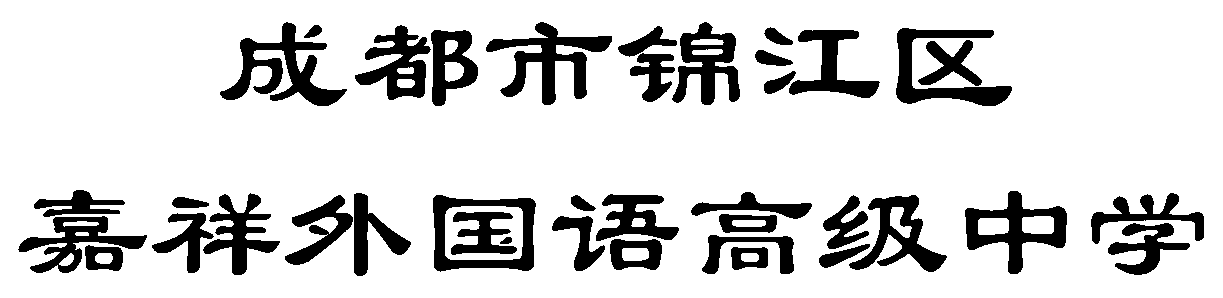
\includegraphics[width=0.6\textwidth]{figures/jxlogo.eps}
  \end{figure}
  \vspace*{21pt}
  \hei\biaotizihao{\textbf{论~文~训~练}}
  \vspace*{52.5pt}

  \begin{figure}[h]
  \centering
  % 
\includegraphics[width=0.3\textwidth]{figures/tjulogo.eps}
  \end{figure}

  \vspace*{5pt}
  \hei\sanhao{\textbf{题目:\@ctitle}}
  \vspace*{16pt}
  
  \vspace*{114pt}
  \renewcommand\arraystretch{1.5}
  \setlength{\@title@width}{5cm}
  {\sanhao\song{\bf{
  \begin{tabular}{lc}
    % 学\qquad 院&  \underline{\makebox[\@title@width][c]{\@caffil}} \\
    % 专\qquad 业 &  \underline{\makebox[\@title@width][c]{\@csubject}} \\
    班\qquad 级  &  \underline{\makebox[\@title@width][c]{\@cgrade}}\\
    姓\qquad 名 &  \underline{\makebox[\@title@width][c]{\@cauthor}} \\
    % 指导教师 &  \underline{\makebox[\@title@width][c]{\@csupervisor}} \\
  \end{tabular}}}
 }
  \vspace*{51.4pt}

\song\sanhao{\textbf{\@cdate}}
\end{center}
\end{titlepage}

%%%%%%%%%%%%%%%%%%%   Abstract and Keywords  %%%%%%%%%%%%%%%%%%%%%%%
\clearpage
\markboth{摘~要}{摘~要}
\pdfbookmark[0]{摘~~要}{cabstract}
%\addcontentsline{toc}{chapter}{摘~要}
%\chapter*{\centering\sanhao\hei\bfseries 摘\qquad 要}
\chapter*{\centering\sanhao\hei 摘\qquad 要}
\song\defaultfont
\@cabstract
\vspace{\baselineskip}

\hangafter=1\hangindent=52.3pt\noindent
{\hei\xiaosi 关键词:} \@ckeywords
\thispagestyle{empty}

%%%%%%%%%%%%%%%%%%%   English Abstract  %%%%%%%%%%%%%%%%%%%%%%%%%%%%%%
\clearpage
%\phantomsection
\markboth{ABSTRACT}{ABSTRACT}
\pdfbookmark[0]{ABSTRACT}{eabstract}
%\addcontentsline{toc}{chapter}{ABSTRACT}
\chapter*{\centering\sanhao{\bf{ABSTRACT}}}
%\vspace{\baselineskip}
\@eabstract
\vspace{\baselineskip}

\hangafter=1\hangindent=60pt\noindent
{\textbf{Keywords:}} \@ekeywords
\thispagestyle{empty}
}
\makeatother
                                 % 完成对论文各个部分格式的设置
\frontmatter                                         % 以下是论文导言部分,包括论文的封面,中英文摘要和中文目录
\fancypagestyle{plain}{
\fancyhf{}
\renewcommand{\headrulewidth}{0 pt}
\fancyfoot[C]{\song\xiaowu~\thepage~}
}
% 直接从 Word 模板生成封面导出 pdf 似乎更方便
% !Mode:: "TeX:UTF-8"

%%  可通过增加或减少 setup/format.tex中的
%%  第274行 \setlength{\@title@width}{8cm}中 8cm 这个参数来 控制封面中下划线的长度。

\cheading{泰勒公式与等价无穷小在物理学中的应用}      % 设置正文的页眉,需要填上对应的毕业年份
\ctitle{泰勒公式与等价无穷小在物理学中的应用}    % 封面用论文标题,自己可手动断行
% \caffil{管理与经济学部} % 学院名称
% \csubject{工业工程}   % 专业名称
\cgrade{六年一贯衔接一班}            % 年级
\cauthor{Johnny}            % 学生姓名
% \cnumber{3012209017}        % 学生学号
% \csupervisor{杨道箭}        % 导师姓名
% \crank{副教授}              % 导师职称

\cdate{\the\year~年~\the\month~月~\the\day~日}

\cabstract{
在数学分析中有一个重要定理,即泰勒公式,该公式将无穷逼近的思想转化为具体的计算方法.物理学中也有很多利用等价无穷小的地方.本文收集了部分物理学中可以直接应用泰勒公式解决的问题,并由泰勒公式证明了一些常用等价无穷小.
}

\ckeywords{泰勒公式;等价无穷小;学科融合}

\eabstract{
In analysis there is a vital theorem, Taylor's theorem. It gives an approximation of a function by calculating the value around a specific point. We also do approximation using equivalent infinitesimal in physics. This thesis concentrates on some of these problems which can be directly solved by Taylor's theorem or can be solved by equivalent infinitesimal. 
}

\ekeywords{Taylor's theorem, equivalent infinitesimal, fusion of subjects}

\makecover

\clearpage
                                % 封面

%%%%%%%%%%   目录   %%%%%%%%%%
\defaultfont
\clearpage{\pagestyle{empty}\cleardoublepage}
\setcounter{page}{1}                                 % 单独从 1 开始编页码
\pagenumbering{arabic}
\titleformat{\chapter}{\centering\sanhao\hei}{\chaptername}{2em}{} % 设置目录两字的格式
\pdfbookmark[0]{目~~录}{mulu}
\tableofcontents                                     % 中文目录
\fancypagestyle{plain}{
\fancyhf{}
\renewcommand{\headrulewidth}{0 pt}
\fancyfoot[C]{\song\xiaowu~\thepage~}
}
\thispagestyle{plain}

\mainmatter\defaultfont\sloppy\raggedbottom
\makeatletter
\fancypagestyle{plain}{                              % 设置开章页眉页脚风格
    \fancyhf{}
    \fancyhead[C]{\song\wuhao \@cheading}            % 首页页眉格式
    \fancyfoot[C]{\song\xiaowu ~\thepage~}           % 首页页脚格式
    \renewcommand{\headrulewidth}{0.5pt}
    \renewcommand{\footrulewidth}{0pt}
}
\makeatother
\setcounter{page}{1}                                 % 单独从 1 开始编页码
\titleformat{\chapter}{\centering\xiaosan\hei}{\chaptername}{2em}{} % 恢复chapter标题格式要求

%%%%%%%%%  正文  %%%%%%%%%
% !Mode:: "TeX:UTF-8"
% !TEX root = tjumain.tex

\iffalse
\bibliography{reference/reference.bib} % 欺骗latextools获取bib文件
\fi

%%%%%%% 正文 %%%%%%%

\chapter{引言}

笔者在学习高中数学时,无意间接触到了Taylor公式.对于这样一个可以用来逼近函数值的定理,笔者好奇其是否能在物理学中有所应用,于是在预习物理时特意留心,注意到了两个可以直接利用Taylor公式(方法)证明的命题,以及若干利用等价无穷小解决的问题.本文简要记录了这些结论.

由于笔者并没有专门研究物理学,本文中的纰漏在所难免,特此致歉.

\chapter{Taylor公式及其证明}

\begin{theorem}{\textbf{带Peano余项的Taylor公式}\cite{ayumu}}
	设函数$f(x)$在$x_0$处有$n$阶导数,则当$x \to x_0$时,$$f(x) = f(x_0) + \frac{1}{1!}f'(x_0)(x-x_0) + \frac{1}{2!}f''(x_0)(x-x_0)^2 + \cdots + \frac{1}{n!}f^{(n)}(x_0)(x-x_0)^n + o[(x-x_0)^n]$$
\end{theorem}
\begin{proof}
	对$n$进行归纳证明:记$$T_{n}(f,x_0;x):=f(x_0) + \frac{1}{1!}f'(x_0)(x-x_0) + \frac{1}{2!}f''(x_0)(x-x_0)^2 + \cdots + \frac{1}{n!}f^{(n)}(x_0)(x-x_0)^n$$
	当$n=1$时,命题即为$$f(x)=f(x_0)+f'(x_0)(x-x_0)+o(x-x_0),~x \to x_0$$
	由无穷小增量公式,该命题成立; \\
	假设当$n=k$时命题成立.由于
	$$T_{k+1}(f,x_0;x)=f(x_0) + \frac{1}{1!}f'(x_0)(x-x_0) + \frac{1}{2!}f''(x_0)(x-x_0)^2 + \cdots + \frac{1}{(k+1)!}f^{(k+1)}(x_0)(x-x_0)^{k+1}$$
	故
	$$T'_{k+1}(f,x_0;x)=f'(x_0) + \frac{1}{1!}f''(x_0)(x-x_0) + \cdots + \frac{1}{k!}f^{(k+1)}(x_0)(x-x_0)^{k} = T_k(f',x_0;x)$$
	由l’Hôpital法则和归纳假设可知$$\lim_{x \to x_0} \frac{f(x)-T_{k+1}(f,x_0;x)}{(x-x_0)^{k+1}} = \frac{1}{k+1} \lim_{x \to x_0} \frac{f'(x)-T_{k}(f',x_0;x)}{(x-x_0)^{k}} = 0$$
	由归纳原理知原命题成立.
\end{proof}

可以认为,Taylor公式通过一个函数在某点附近的信息来估计函数值.更确切地说,它通过一个多项式拟合原函数.

在应用Taylor公式时,我们倾向于尽可能多地简化该式子.令$x_0=0$,即得到\textbf{Maclaurin公式}.

\begin{corollary}{\textbf{Maclaurin公式}}
	设函数$f(x)$在$0$处有$n$阶导数,则当$x \to 0$时,$$f(x)=f(0)+\frac{f'(0)}{1!}x + \frac{f''(0)}{2!}x^2 + \cdots + \frac{f^{(n)}(0)}{n!}x^n + o(x^n)$$
\end{corollary}

微元法中应用的“等价无穷小”本质上就是Maclaurin公式.因而在后文主要讨论的都是该公式的应用.


\chapter{Taylor公式(方法)在物理学中的直接应用}

\section{推导变速直线运动公式}

先来看一个简单的结论.在匀变速直线运动中,位移关于时间的函数$x(t)$满足$$x(t) = x_0 + v_0t + \frac{1}{2}at^2$$
我们好奇能否将这个形式进行推广?如果知道物体在$0$时刻处的速度、加速度、加速度的变化率、加速度的变化率的变化率$\cdots$能否给出$x(t)$的表达式?

注意到,上式与Maclaurin公式的形式很像.若设$x(t)$表示在直线运动中从$0$时刻到$t$时刻中物体的位移量,这意味着$$x(t) = x(0) + \frac{1}{1!} x'(0)t + \frac{1}{2!} x''(0)t^2$$
然而这个形式不完全等价于Maclaurin公式,因为该公式的效用极限过程是$t \to 0$.换个思路,我们可以用接近于Taylor公式证明的方法来证明该加强命题:

\begin{proposition}{}
	设$a_i~(i=0,1,2,\cdots)$为常数,在$x(t)$的某一阶导函数为常值函数时,有$$x(t) = \sum_{i=0}^{\infty} a_ix^{(i)}(0) t^{i} = a_0x(0) + a_1x'(0)t + a_2x''(0)t^2 + \cdots$$
	其中$\{ a_n \}_{n=0}^{\infty}$满足$a_n = \dfrac{1}{n!}$.
\end{proposition}
\begin{remark}
	该命题的形式与Legendre定理类似.因为对任意$n>N$都有$x^{(n)}(0)=0$,故这是个有限项多项式.
\end{remark}
\begin{remark}
	若$x(t)$不存在任一阶导函数为常值函数,可以取某个足够大的$n$来近似计算.
\end{remark}
\begin{proof}
	设$x(t)$的第$n$阶导函数为常值函数,对$n$进行归纳证明.记$$T_n(x;t) := x(t) = x(0) + \frac{1}{1!} x'(0)t + \frac{1}{2!} x''(0)t^2 + \cdots + \frac{1}{n!} x^{(n)}(0)t^n$$
	$1^{\circ}~$当$n=1$时,由于此时物体作匀速直线运动,$x(t)=x(0)+x'(0)t$自然成立. \\
	$2^{\circ}~$假设$n=k$时命题成立.在$n=k+1$时,由于
	$$T_{k+1}(x;t) = x(0) + \frac{1}{1!} x'(0)t + \frac{1}{2!} x''(0)t^2 + \cdots + \frac{1}{(k+1)!} x^{(k+1)}(0)t^{k+1}$$
	$$T'_{k+1}(x;t) = x'(0) + \frac{1}{1!} x''(0)t + \frac{1}{2!} x'''(0)t^2 + \cdots + \frac{1}{k!} x^{(k+1)}(0)t^k = T_{k}(x';t)$$
	由归纳假设,$T_k(x',t)=x(t)$.故$x(t)=T_{k+1}(x;t)$. \\
	由数学归纳原理可知命题成立.
\end{proof}

命题3.1提供了一个有趣的直觉:如果能搞清楚某物体任一时间下的运动状态,我们就能推导它的运动全程.这个直觉被应用在了刘慈欣的科幻小说《镜子》\cite{liucixin}中:文中气象模拟员白冰通过对宇宙大爆炸时有限个物理量的控制模拟出了我们的宇宙.不过显然对于一个混沌系统不能这么搞.

\section{推导近地重力势能公式}

上一小节似乎是杀鸡用了牛刀.本小节更能体现出Taylor公式在处理近似时的重要作用.

\begin{proposition}
	在选取地表为零势能点时,近地物体的重力势能为$$E_{PG} \approx mgh$$
\end{proposition}
\begin{remark}
	当物体的质量到达天文质量级时,这个估计将会极不准确,因而只讨论物体质量远小于地球质量的情况.
\end{remark}

对于一个近地物体,设地球半径$R$,地表与该物体距离$h$,地球、该物体质量分别为$M,m$,$G$为万有引力常数,选择无穷远处为势能零点,则该物体的引力势能为(将其看做关于$h$的函数)$$E_P(h) = - \frac{GMm}{R+h}$$
由于$h \ll R$,令$h \to 0$,由Maclaurin公式,此时有
\begin{align*}
	E_P(h) &= E_P(0)+\frac{E'_P(0)}{1!}h + o(h^2) \\
	&\approx -\frac{GMm}{R} + \frac{GMm}{R^2} h
\end{align*}
由黄金代换公式,$$E_P(h) \approx -\frac{GMm}{R} + mgh$$
注意到这个式子的势能零点是无穷远处,而近地重力势能的势能零点是地表.这两个零势能点的势能差值等于地表处因(近似等价于)球心的万有引力而具有的势能(此时零势能点为无穷远处),这个值恰好为$$-\frac{GMm}{R}$$
于是近地处物体重力势能为(零势能点为地表)$$E_{PG} \approx mgh$$

\chapter{等价无穷小的应用}

由Maclaurin公式,可以得到以下重要的等价无穷小:

\begin{proposition}
	当$x \to 0$时, 
	$$(1+x)^{\alpha} -1 \sim \alpha x, \qquad \sin x \sim x \sim\tan x, \qquad 1-\cos x \sim \dfrac{x^2}{2}$$
\end{proposition}

这些结论是显而易见的.



\begin{example}
	如图i所示,岸上一小人以恒定速度$v$拉动绳子的一头,船上的小人抓住绳子的另一头,求船速$v'$.
	
	\begin{center}
		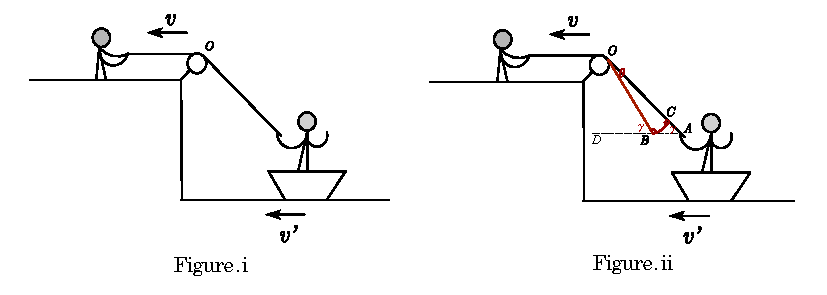
\includegraphics[width=14cm]{4.1.pdf}
	\end{center}
\end{example}
\begin{solution}
	如图ii所示,在一段极短的时间$\Delta t$内,设绳子的一头从$A$移动到$B$,过点$B$作$BC \bot OB$. \\
	在$\vartriangle OBC$中,由于$\tan \theta \sim \sin \theta$,又$BC = \tan \theta OB = \sin \theta OC$,故可看做$OC=OB=l$,此时$\angle OBC = 90^{\circ}$.同理可知$\angle OCB = 90^{\circ}$.于是$\overset{\LARGE{\frown}}{BC} = \theta l = \tan \theta l = BC$,可将$\overset{\LARGE{\frown}}{BC}$看做直线. \\
	考虑$\angle OBD=\gamma$,于是$\angle CBA=90^{\circ} - \gamma$,那么$\angle CAB = \gamma$.在直角三角形$\vartriangle ABC$中,$AB = v' \Delta t$,$AC = v \Delta t$,故$v \Delta t = \cos \gamma v' \Delta t$,解得$v' = \dfrac{v}{\cos \gamma}$.
\end{solution}





%%%%%%% 结论 %%%%%%%

\addcontentsline{toc}{chapter}{结\quad 论} %添加到目录中

\chapter*{结\quad 论}

逸一时,误一世。逸久逸久,罢已龄!


%%%%%%%%%%  参考文献  %%%%%%%%%%
\defaultfont
% \bibliographystyle{references/ref.buk}
\bibliographystyle{plain}
\phantomsection
\markboth{参考文献}{参考文献}
\addcontentsline{toc}{chapter}{参考文献}       % 参考文献加入到中文目录
\nocite{*}                                     % 若将此命令屏蔽掉,则未引用的文献不会出现在文后的参考文献中
\bibliography{references/reference.bib}
\titleformat{\chapter}{\centering\sihao\hei}{\chaptername}{2em}{}
% % !Mode:: "TeX:UTF-8"

\titlecontents{chapter}[2em]{\vspace{.5\baselineskip}\xiaosan\song}%
             {\prechaptername\CJKnumber{\thecontentslabel}\postchaptername\qquad}{} %
             {}             % 设置该选项为空是为了不让目录中显示页码
\addcontentsline{toc}{chapter}{外文资料}
%\setcounter{page}{1}       % 如果需要从该页开始从 1 开始编页,则取消该注释
\markboth{外文资料}{外文资料}
\chapter*{外文资料}

Here follows the English paper.

...              % 外文资料
% % !Mode:: "TeX:UTF-8"

\titlecontents{chapter}[2em]{\vspace{.5\baselineskip}\xiaosan\song}
             {\prechaptername\CJKnumber{\thecontentslabel}\postchaptername\qquad}{}
             {}             % 设置该选项为空是为了不让目录中显示页码
\addcontentsline{toc}{chapter}{中文译文}
\setcounter{page}{1}            % 单独从 1 开始编页码
\markboth{中文译文}{中文译文}   % 用于将章节号添加到页眉中
\chapter*{中文译文}

这里就是外文资料的中文翻译。

...
              % 中文译文
% !Mode:: "TeX:UTF-8"

\titlecontents{chapter}[2em]{\vspace{.5\baselineskip}\xiaosan\song}
             {\prechaptername\CJKnumber{\thecontentslabel}\postchaptername\qquad}{} 
             {}                            % 设置该选项为空是为了不让目录中显示页码
\fancypagestyle{plain}   % 设置页眉页脚风格,按照教务处规定,此处出现页眉,但是没有页脚(页码)。
\lhead{}
\rhead{}
\chead{\song\wuhao 泰勒公式与等价无穷小在物理学中的应用} % 设置页眉内容
\lfoot{}
\cfoot{}
\rfoot{}
\markboth{致\quad 谢}{致\quad 谢}
\addcontentsline{toc}{chapter}{致\quad 谢} % 添加到目录中
\chapter*{致\quad 谢}
\setcounter{page}{1}

\begin{itemize}
	\item 感谢\textsc{Roger Tang}老师,没有他要求的寒假作业就没有我对于此问题的深入思考.
	\item 感谢\href{https://www.overleaf.com/latex/templates/xi-nan-da-xue-swu-beamer-zhu-ti/bgprxfbyhqsb}{LIU Qilong}与\href{https://www.overleaf.com/latex/templates/tian-jin-da-xue-tianjin-university-tju-2022ben-ke-sheng-bi-ye-lun-wen/rrfbkrpsrdkh}{Someone}提供的精美\LaTeX 模版.
	\item 感谢\href{https://www.overleaf.com/}{Overleaf}提供的方便快捷\LaTeX 编辑流程.
\end{itemize}
            % 致谢
\clearpage
\end{document}                                 % 结束全文
